% !TeX root = Protokoll.tex
\subsection{Quantenzahlen des Wasserstoffs}
Ein Atom mit einem Elektron, wird durch die Quantenzahlen, die Hauptquantenzal $n$, die Drehimpulsquantenzahl $l$, die Magnetquantenzahl $m$ sowie den Spin $s$ beschrieben.\\
Der Bahndrehimpuls des Elektrons ruft ein magnetisches Moment hervor, allerdings lässt sich auch bei Systemen mit verschwindendem Bahndrehimpuls ein magnetisches Moment nachweisen. 
Dies kann so interpretiert werden, dass das Elektron einen Eigenendrehimpuls besitzt, 
der als Spin $s$ bezeichnet wird.\\
Mithilfe der Wahrscheinlichkeitsstromdichte $j$ der Wellenfunktion eines Wasserstoffatoms lässt sich
\begin{align}
	\mu_z=-e_0\int j df=-\frac{1}{2}\frac{e_0}{m_0}\hbar m \int\limits_{0}^{\pi}\int\limits_{0}^{\infty} R^2(r)\Theta^2(\theta)r^2\sin\theta drd\theta
\end{align}
bestimmen. 
Dabei ist $\mu_z$ das magnetische Moment in $z$-Richtung, $df$ die Flächenstück in Kugelkoordinaten, $e_0$ die Elementarladung, $R(r)$ ist der Radialanteil der Wellenfunktion und $\Theta(\theta)$ der Breitenkreisanteil der Wellenfunktion.
Nach ausgeführter Integration ergibt sich unter Berücksichtigung der Normierung von $R(r)$ und $\Theta(\theta)$  
\begin{equation}
	\mu_z=-\frac{1}{2}\frac{e_o}{m_0}\hbar m.
\end{equation}
Darin ist $m_0$ die Masse eines Elektrons und $\hbar$ das Planksche Wirkungsquantum und $m$ die zuvor erwähnte Quantenzahl. 
Das magnetische Moment kann in Einheiten des Bohrschen Magnetons $\mu_B$ angegeben werden.
\begin{align}
	\mu_z &= \mu_B m\\
	\mu_B:&=-\frac{1}{2}\frac{e_0}{m_0}\hbar
\end{align}
\subsection{Energieaufspaltung durch ein externes Magnetfeld}
Befindet sich das System in einem Magnetfeld so richtet sich der Drehimpuls aus.
Das Magnetfeld soll entlang der $z$-Achse herrschen, dann gilt für die $z$ Komponente des Drehimpulses
\begin{align}
	l_z=m_l\hbar.
\end{align}
Eine einzelne Komponente eines Vektors kann nur kleiner gleich dem Betrag des Vektors sein, daher ergeben sich für die Orientierungsquantenzahl
$m_l$ die möglichen Werte 
\begin{align}
	m_l = l,\ l-1,\ ...,\ 1,\ 0,\ -1,\ ... ,\ -l+1,\ -l.
\end{align}
Entsprechend gibt es $2l+1$ Möglichkeiten den Bahndrehimpuls relative zu dem anliegenden Feld auszurichten.
Die Energie eines magnetischen Feldes $E_\text{mag}$ lässt sich mithilfe des magnetischen Momentes des Atoms $\vec{M}$ und der magnetischen Feldstärke eines homogenen externen Magnetfeldes $\vec{B}$ kann durch 
\begin{align}
	E_\text{mag}=\vec{M}\cdot\vec{B}=\mu_zB=m_l\ \mu_B\ B\label{eq:Emag}
\end{align}
beschrieben werden. 
Daraus folgt das die Energie $E_0$ in $2l+1$ Niveaus aufspaltet.
\begin{wrapfigure}{r}{0.5\textwidth}
	\centering
	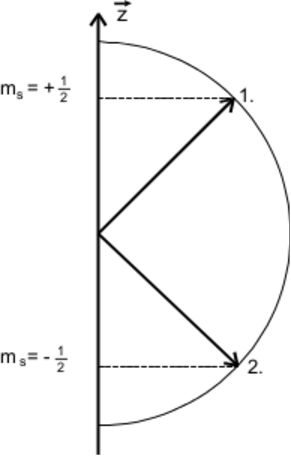
\includegraphics[width=\textwidth/4]{../Grafiken/SpinElektron.pdf}
	\caption{Die Ausrichtung des Elektronen Spins bei angeschaltetem Magnetfeld.\cite{V28}}\label{fig:ResonanzTheo}
\end{wrapfigure}
Wenn allerdings ein Elektron ohne einen Bahndrehimpuls sich in einem Magnetfeld befindet, wird eine Aufspaltung in zwei Energieniveaus beobachtet, daraus lässt sich schließen das die Elektronen einen Spin besitzen und das dieser $\frac{1}{2}$ beträgt, eine Veranschaulichung ist in \cref{fig:ResonanzTheo} dargestellt.
Interessant ist das magnetische Moment $\mu_{s_z}$ das durch den Spin hervorgerufen wird zu beschreiben.
\begin{align}
	\mu_{s_z}=-g\frac{1}{2}\mu_B\label{eq:musz}
\end{align}
Dabei ist $g$ der Landé-Faktor oder auch gyromagnetisches  Verhältnis genannt und wird eingeführt weil der Zusammenhang zwischen Spin und magnetischem Moment anders sein kann als beim Bahndrehimpuls. Der Wert dieses Faktors $g$ soll in diesem Versuch bestimmt werden.

\subsection{Elektronenspinresonanz}

In diesem Versuch wird zur Bestimmung des gyromagnetischen Verhältnis das Verfahren der Hochfrequenz-Spektroskopie verwendet.
Es wird eine Substanz, hier Diphenylpikrylhydrazyl, die praktisch freie Elektronen enthält in ein homogenes Magnetfeld eingebracht. Dieses 
spaltet das Energieniveau des Elektrons auf. Aufgrund des Spins $s = \tfrac{1}{2}$ des Elektrons entstehen so zwei Energieniveaus.%, wie in 
%\cref{fig:Aufspaltung} gezeigt.
%TODO Neue Seite
\newpage
\begin{wrapfigure}{r}{0.5\textwidth}
	\centering
	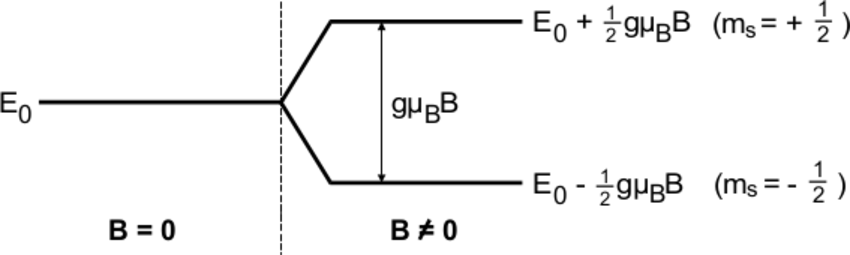
\includegraphics[width=0.5\textwidth]{../Grafiken/EnergieAufspaltung.pdf}
	\caption{Darstellung der Energieaufspaltung der Energie eines Elektrons durch ein externes Magnetfeld.\cite{V28}}\label{fig:Aufspaltung}
\end{wrapfigure}
Die Differenz der beiden Niveaus ist dabei 
\begin{align}
	\Delta E = g\ \mu_B \ B.
\end{align}
Dies folgt aus Gleichung \eqref{eq:Emag} und \eqref{eq:musz} dies ist in \cref{fig:Aufspaltung} veranschaulicht.
Aus der Maxwell-Boltzmann-Statistik folgt, dass das obere Energieniveau schwächer besetzt ist als das untere.
Werden dem System jetzt Photonen mit der Energie
\begin{align}
	\Delta E = h\nu
	\label{eq:energie}
\end{align}
zugeführt, wechseln die Elektronen in das höhere Energieniveau und klappen ihren Spin um.
Dieser Prozess wird Elektronenspinresonanz genannt.
Die bei diesem Vorgang aufgenommene Energie geben die Elektronen durch Wechselwirkungsprozesse wieder ab. 

{ %TODO: Alte Version
%wechseln die Elektronen das Energieniveau in ein höheres und klappen ihren Spin um.

% Anmerkung: Das stimmt nicht, wir haben nur 10 - 30 MHz und es hat trotzdem funktioniert.
%Damit die Photonen diese Energie besitzen, müssen sie eine Frequenz $\nu$ in Größenordnung von 
%\SI{140}{\mega\hertz} besitzen.
% Anmerkung: Die Aufnahme der Energie und das Unklappen ist die SpinResonanz nicht die Abgabe der Energie.
%Die Elektronen geben ihre Energie durch Wechselwirkungsprozesse wieder ab. Dieser Prozess wird Elektronenspinresonanz genannt.	
}


